%%%%%%%%%%%%%%%%%%%%%%%%%%%%%%%%%%%%%%%%%%%%%%%
%%%     Declarations (skip to Begin Document, line 88, for parts you fill in)
%%%%%%%%%%%%%%%%%%%%%%%%%%%%%%%%%%%%%%%%%%%%%%%

\documentclass[10pt]{article}

\usepackage{geometry}  % Lots of layout options.  See http://en.wikibooks.org/wiki/LaTeX/Page_Layout
\geometry{letterpaper}  % ... or a4paper or a5paper or ... 
\usepackage{fullpage}  % somewhat standardized smaller margins (around an inch)
\usepackage{setspace}  % control line spacing in latex documents
\usepackage[parfill]{parskip}  % Activate to begin paragraphs with an empty line rather than an indent

\usepackage{amsmath,amssymb}  % latex math
\usepackage{empheq} % http://www.ctan.org/pkg/empheq
\usepackage{bm,upgreek}  % allows you to write bold greek letters (upper & lower case)

% allows strikethroughs in math via \cancel{math text goes here}
\usepackage{cancel}

% for typsetting algorithm pseudocode see http://en.wikibooks.org/wiki/LaTeX/Algorithms_and_Pseudocode
\usepackage{algorithmic,algorithm}  

\usepackage{graphicx}  % inclusion of graphics; see: http://en.wikibooks.org/wiki/LaTeX/Importing_Graphics
% allow easy inclusion of .tif, .png graphics
\DeclareGraphicsRule{.tif}{png}{.png}{`convert #1 `dirname #1`/`basename #1 .tif`.png}

% \usepackage{subfigure}  % allows subfigures in figure
\usepackage{caption}
\usepackage{subcaption}
\usepackage{verbatim}

\usepackage{xspace}
\newcommand{\latex}{\LaTeX\xspace}

\usepackage{xcolor}  % http://en.wikibooks.org/wiki/LaTeX/Colors

\long\def\todo#1{{\color{orange}{\bf TODO: #1}}}

\long\def\ans#1{{\color{blue}{\em #1}}}
\long\def\ansnem#1{{\color{blue}#1}}
\long\def\boldred#1{{\color{red}{\bf #1}}}
\long\def\boldred#1{\textcolor{red}{\bf #1}}
\long\def\boldblue#1{\textcolor{blue}{\bf #1}}

% Useful package for syntax highlighting of specific code (such as python) -- see below
\usepackage{listings}  % http://en.wikibooks.org/wiki/LaTeX/Packages/Listings
\usepackage{textcomp}

%%% The following lines set up using the listings package
\renewcommand{\lstlistlistingname}{Code Listings}
\renewcommand{\lstlistingname}{Code Listing}

%%% Specific for python listings
\definecolor{gray}{gray}{0.5}
\definecolor{green}{rgb}{0,0.5,0}

\lstnewenvironment{python}[1][]{
\lstset{
language=python,
basicstyle=\footnotesize,  % could also use this -- a little larger \ttfamily\small\setstretch{1},
stringstyle=\color{red},
showstringspaces=false,
alsoletter={1234567890},
otherkeywords={\ , \}, \{},
keywordstyle=\color{blue},
emph={access,and,break,class,continue,def,del,elif ,else,%
except,exec,finally,for,from,global,if,import,in,i s,%
lambda,not,or,pass,print,raise,return,try,while},
emphstyle=\color{black}\bfseries,
emph={[2]True, False, None, self},
emphstyle=[2]\color{green},
emph={[3]from, import, as},
emphstyle=[3]\color{blue},
upquote=true,
morecomment=[s]{"""}{"""},
commentstyle=\color{gray}\slshape,
emph={[4]1, 2, 3, 4, 5, 6, 7, 8, 9, 0},
emphstyle=[4]\color{blue},
literate=*{:}{{\textcolor{blue}:}}{1}%
{=}{{\textcolor{blue}=}}{1}%
{-}{{\textcolor{blue}-}}{1}%
{+}{{\textcolor{blue}+}}{1}%
{*}{{\textcolor{blue}*}}{1}%
{!}{{\textcolor{blue}!}}{1}%
{(}{{\textcolor{blue}(}}{1}%
{)}{{\textcolor{blue})}}{1}%
{[}{{\textcolor{blue}[}}{1}%
{]}{{\textcolor{blue}]}}{1}%
{<}{{\textcolor{blue}<}}{1}%
{>}{{\textcolor{blue}>}}{1},%
%framexleftmargin=1mm, framextopmargin=1mm, frame=shadowbox, rulesepcolor=\color{blue},#1
framexleftmargin=1mm, framextopmargin=1mm, frame=single,#1
}}{}
%%% End python code listing definitions

\DeclareMathOperator{\diag}{diag}
\DeclareMathOperator{\cov}{cov}

%%%%%%%%%%%%%%%%%%%%%%%%%%%%%%%%%%%%%%%%%%%%%%%
%%%     Begin Document
%%%%%%%%%%%%%%%%%%%%%%%%%%%%%%%%%%%%%%%%%%%%%%%

\begin{document}

\begin{center}
    {\Large {\bf ISTA 421/521 -- Homework 5}} \\
    \boldred{Due: Wednesday, December 5, 5pm} \\
    20 pts total for Undergrads, 24 pts total for Grads\\
    
\end{center}

\begin{flushright}
Ken Youens-Clark

Graduate 
\end{flushright}

\vspace{1cm}
{\Large {\bf Instructions}}

In this assignment, exercises 5 and 6 require you to write small python scripts; the details for those scripts, along with their .py name are described in the exercises.  All of the exercises in this homework require written derivations, short answers, and/or plots, so you will also submit a .pdf of your written answers.  (You can use \latex or any other system (including handwritten; plots, of course, must be program-generated) as long as the final version is in PDF.)

\boldred{The final submission will include (minimally) the two scripts you need to write for problems 5 and 6, and a PDF version of your written part of the assignment.  You are required to create either a .zip or tarball (.tar.gz / .tgz) archive of all of the files for your submission and submit your archive to the d2l dropbox by the date/time deadline above.}

NOTE: Problem 3 is required for Graduate students only; Undergraduates may complete this problem for extra credit equal to the point value.

(FCMA refers to the course text: Rogers and Girolami (2016), {\em A First Course in Machine Learning}, second edition.  For general notes on using \latex to typeset math, see: \\{\tt http://en.wikibooks.org/wiki/LaTeX/Mathematics})
\vspace{.5cm}



%%%%%%%%%%%%%%%%
%%%     Problems
%%%%%%%%%%%%%%%%

\newpage
\begin{itemize}

%%%     Problem 1
\item[1.]  [5 points]  %\boldred{Required only for Graduates}
Adapted from {\bf Exercise 5.3} of FCMA p.202:

Compute the maximum likelihood estimates of $\boldsymbol{\mu}_c$ and $\boldsymbol{\Sigma}_c$ for class $c$ of a Bayesian classifier with Gaussian class-conditionals and a set of $N_c$ objects belonging to class $c$, $\mathbf{x}_1$, ..., $\mathbf{x}_{N_c}$. 

{\bf Solution.} 

\begin{eqnarray*}
\begin{aligned}
%
% Likelihood
%
\text{Likelihood}
\\
L &= p(\mathbf{X}^c|\boldsymbol{\mu}_c, \boldsymbol{\Sigma}_c)
\\
\text{is product of (Gaussian) probabilities}
\\
&= \prod_n^N \mathcal{N} (\mathbf{x}_n|\boldsymbol{\mu}_c, \boldsymbol{\Sigma}_c)
\\
&= \prod_n^N 
\frac{1}{(2 \pi)^{N/2} | \boldsymbol {\Sigma}_c |^{1/2}} 
\exp 
\left\{ 
-\frac{1}{2} (\mathbf{x}_n\ - \boldsymbol {\mu}_c)^\top \boldsymbol {\Sigma}_c^{-1} (\mathbf{x}_n - \boldsymbol {\mu}_c)
\right\}
\\
&\propto 
|\boldsymbol {\Sigma}_c|^{-{N_c}/2}
\exp 
\left\{ 
\sum_n^{N_c} -\frac{1}{2} (\mathbf{x}_n\ - \boldsymbol {\mu}_c)^\top \boldsymbol {\Sigma}_c^{-1} (\mathbf{x}_n - \boldsymbol {\mu}_c)
\right\}
\\
% 
% Log
%
\text{Use log to handle exponent}
\\
\log(L) &= 
\left( - \frac{N_c}{2} \log(|\boldsymbol {\Sigma}_c|) \right)
\left(
-\frac{1}{2} \sum_n^{N_c} (\mathbf{x}_n\ - \boldsymbol {\mu}_c)^\top \boldsymbol {\Sigma}_c^{-1} (\mathbf{x}_n - \boldsymbol {\mu}_c)
\right)
\end{aligned}
\end{eqnarray*}

\begin{eqnarray*}
\begin{aligned}
%
% Derivative \mu
%
\text{Take derivative w.r.t. $\boldsymbol \mu_c$}
\\
\frac{\partial \log(L)}{\partial \boldsymbol \mu_c} 
&= -\frac{1}{2} \sum_n^{N_c} 2 \boldsymbol {\Sigma}_c^{-1} (\mathbf{x}_n - \boldsymbol {\mu}_c) 
\\
&= - \sum_n^{N_c} \boldsymbol {\Sigma}_c^{-1} (\mathbf{x}_n - \boldsymbol {\mu}_c) = 0
\\
\sum_n^{N_c} \boldsymbol {\Sigma}_c^{-1} \boldsymbol {\mu}_c - \sum_n^{N_c} \boldsymbol {\Sigma}_c^{-1} \mathbf{x}_n  &= 0
\\
\boldsymbol {\Sigma}_c^{-1} N_c \boldsymbol {\mu}_c - \boldsymbol {\Sigma}_c^{-1} \sum_n^{N_c} \mathbf{x}_n &= 0
\\
\boldsymbol {\Sigma}_c^{-1} N_c \boldsymbol {\mu}_c &= \boldsymbol {\Sigma}_c^{-1} \sum_n^{N_c} \mathbf{x}_n
\\
N_c \boldsymbol {\mu}_c &= \sum_n^{N_c} \mathbf{x}_n
\\
\boldsymbol {\mu}_c &= \frac{1}{N_c} \sum_n^N  \mathbf{x}_n 
\end{aligned}
\end{eqnarray*}

\begin{eqnarray*}
\begin{aligned}
%
% Derivative \Sigma
%
\text{Take derivative w.r.t. $\boldsymbol {\Sigma}_c$, set to zero, solve}
\\
\frac{\partial \log(L)}{\partial \boldsymbol {\Sigma}_c} 
&=
- \frac{N_c}{2} ( \boldsymbol {\Sigma}_c ^{-1} )
+ \frac{1}{2} 
\sum_n^{N_c} (\mathbf{x}_n\ - \boldsymbol {\mu}_c)^\top \boldsymbol {\Sigma}_c^{-2} (\mathbf{x}_n - \boldsymbol {\mu}_c) = 0
\\
\frac{N_c}{2} ({ \boldsymbol {\Sigma}_c }^{-1}) &=
\frac{1}{2} 
\sum_n^{N_c} (\mathbf{x}_n\ - \boldsymbol {\mu}_c)^\top \boldsymbol {\Sigma}_c^{-2} (\mathbf{x}_n - \boldsymbol {\mu}_c)
\\
N_c ({ \boldsymbol {\Sigma}_c }^{-1}) &= 
\boldsymbol {\Sigma}_c^{-1} \left(
\sum_n^{N_c} (\mathbf{x}_n\ - \boldsymbol {\mu}_c)^\top  (\mathbf{x}_n - \boldsymbol {\mu}_c) 
\right) \boldsymbol {\Sigma}_c^{-1}
\\
N_c \cancel{ ({ \boldsymbol {\Sigma}_c }^{-1}) ({ \boldsymbol {\Sigma}_c }^{-1}) } &= 
\boldsymbol {\Sigma}_c^{-1} \left(
\sum_n^{N_c} (\mathbf{x}_n\ - \boldsymbol {\mu}_c)^\top  (\mathbf{x}_n - \boldsymbol {\mu}_c) 
\right)
\cancel{ \boldsymbol {\Sigma}_c^{-1} ({ \boldsymbol {\Sigma}_c }^{-1}) }
\\
\cancel{ \frac{1}{N_c} N_c } ({ \boldsymbol {\Sigma}_c }^{-1}) &= 
\frac{1}{N_c}
\cancel{ ({ \boldsymbol {\Sigma}_c }^{-1}) \boldsymbol {\Sigma}_c^{-1} }
\left( \sum_n^{N_c} (\mathbf{x}_n\ - \boldsymbol {\mu}_c)^\top  (\mathbf{x}_n - \boldsymbol {\mu}_c) \right) 
\\
{ \boldsymbol {\Sigma}_c }^{-1} &= 
\frac{1}{N_c} \left( \sum_n^{N_c} (\mathbf{x}_n\ - \boldsymbol {\mu}_c)^\top  (\mathbf{x}_n - \boldsymbol {\mu}_c) \right) 
\end{aligned}
\end{eqnarray*}

%%%     Problem 2
\item[2.]  [4 points]
Adapted from {\bf Exercise 5.4} of FCMA p.204:

Compute the maximum likelihood estimates of $q_{mc}$ for class $c$ of a Bayesian classifier with multinomial class-conditionals and a set of $N_c$, $M$-dimensional objects belonging to class $c$: $\mathbf{x}_1, ..., \mathbf{x}_{N_c}$.

{\bf Solution.} %$<$Solution goes here$>$

\begin{eqnarray*}
\begin{aligned}
L &= P(x_n | \mathbf{q})
\\
&= \left( \frac{s_n !}{\prod_{m=1}^M x_{nm} !} \right)
\prod_{m=1}^M {q_m}^{x_{nm}}
\\
\text{Yada yada yada...}
\\
q_{cm} &= \frac{ \sum_{n=1}^{N_c} x_{nm} } { \sum_{m'=1}^M \sum_{n=1}^{N_c} x_{nm'} }
\end{aligned}
\end{eqnarray*}


%%%     Problem 3
\item[3.]  [4 points]  \boldred{Required only for Graduates}
Adapted from {\bf Exercise 5.5} of FCMA p.204:

For a Bayesian classifier with multinomial class-conditionals with $M$-dimensional parameters $\mathbf{q}_c$, compute the posterior Dirichlet for class $c$ when the prior over $\mathbf{q}_c$ is a Dirichlet with constant parameter $\alpha$ and the observations belonging to class $c$ are the $N_c$ observations $\mathbf{x}_1, ..., \mathbf{x}_{N_c}$.

{\bf Solution.} %$<$Solution goes here$>$

\begin{eqnarray*}
\begin{aligned}
L(\mathbf{X}, \mathbf{q}) \propto \prod_{m=1}^M q_m^{x_{nm}}
\end{aligned}
\end{eqnarray*}

%%%     Problem 4
\item[4.]  [3 points]
For a support vector machine, if we remove one of the support vectors from the training set, does the size of the maximum margin decrease, stay the same, or increase for that dataset?  Why?  Also justify your answer by providing a simple dataset (no more than 2-dimensions) in which you identify the support vectors, draw the location of the maximum margin hyperplane, remove one of the support vectors, and draw the location of the resulting maximum margin hyperplane.  Drawing this by hand is sufficient.

{\bf Solution.}

I think by definition the margin must increase if you remove one of the supports from a SVM. As demonstrated by the below examples, the margin is maximized according to the support vectors, and removing one support means the margin is maximized again, necessarily to a larger space. It is not only the width that can change, but, as shown in the second example, the direction/slope of the boundary can be greatly changed by the removal.

\begin{figure}[H]
\centering
  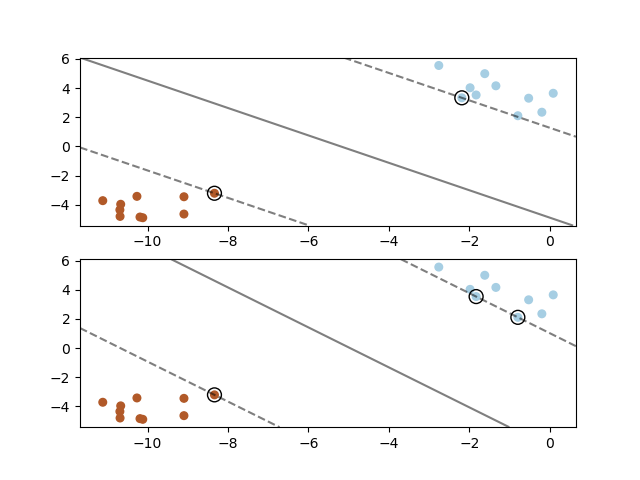
\includegraphics[width=\linewidth]{code/svm.png}
 \caption{Affect on Support Vector Machine of removing one support (random seed = 1)}
\label{label}
\end{figure}

\begin{figure}[H]
\centering
  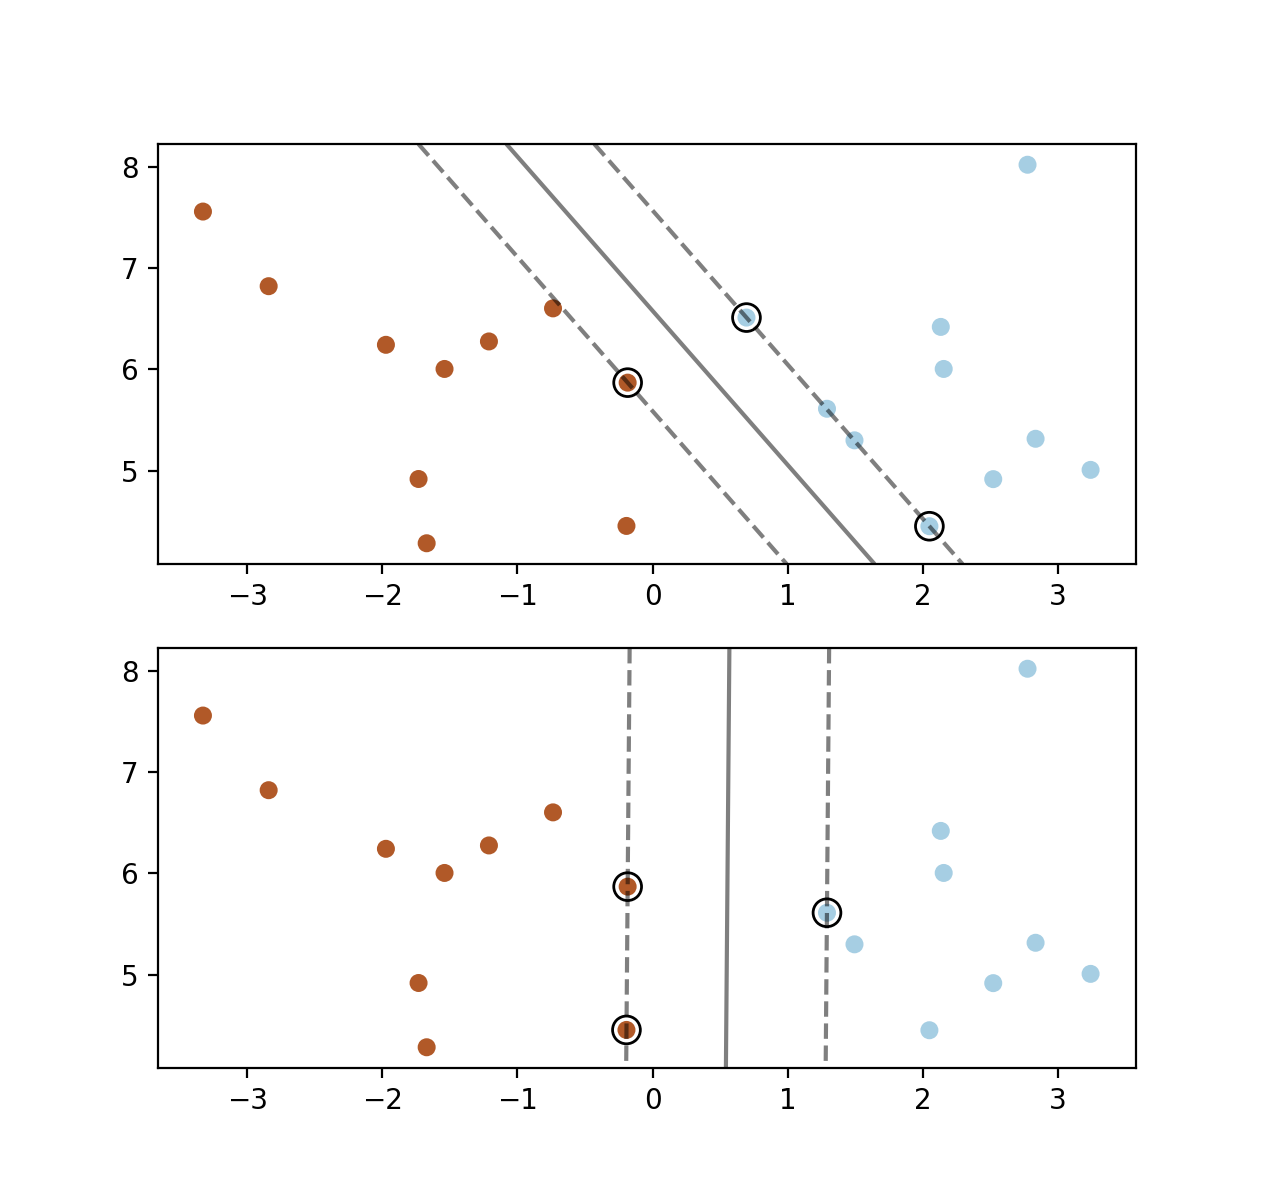
\includegraphics[width=\linewidth]{code/svm2.png}
 \caption{Affect on Support Vector Machine of removing one support (image generated at random, unknown seed)}
\label{label}
\end{figure}

\verbatiminput{./code/svm.py}

%%%     Problem 5
\item[5.]  [4 points]
In this exercise you will use the python script, {\tt knn.py}, which contains code to plot the decision boundary for a k-nearest neighbors classifier.  Two data sources are also provided in the {\tt data} directory: {\tt knn\_binary\_data.csv} and {\tt knn\_three\_class\_data.csv}.

In python file, the function {\tt knn} is to compute the k-nearest neighbors classification for a point {\tt p}, but the functionality is not currently implemented.  You \emph{can} run the code in its unimplemented state, but the decision boundary will not display (everything will be considered the same class).  You must implement this yourself.  Use a Euclidean distance measure for determining the neighbors (note: you don' t need to take the square root! The sum of squares is sufficient).  You do not need to implement any fancy indexing -- you can simply search for the k nearest points by searching over the pairwise distance of the input ({\tt p}) to all of the "training" inputs ({\tt x}).  Use the maximum class frequency as the class decision rule.  You do not need to worry about doing anything special for breaking ties.  The numpy function {\tt argsort} and the python {\tt collections.Counter} may be of use, but are not required.  Submit the {\tt knn.py} file with your implementation.  In your written solution, run the code on both of the provided data sources ( {\tt knn\_binary\_data.csv} and {\tt knn\_three\_class\_data.csv}.), and for each, plot the decision boundary for $k = \{1, 5, 10, 59\}$.  Include informative captions and describe any patterns you see in the decision boundaries as k changes.

{\bf Solution.}

When k=1, the boundaries are too close, creating islands of the green squares when they ought to be assumed to have crossed into enemy territory. K of 5 or 10 does a much better job capturing what I would judge to be the real boundary. K of 59 is far too high and pushes the border too far into green square's territory because there are fewer of those class than the other.

\begin{figure}[H]
\centering
  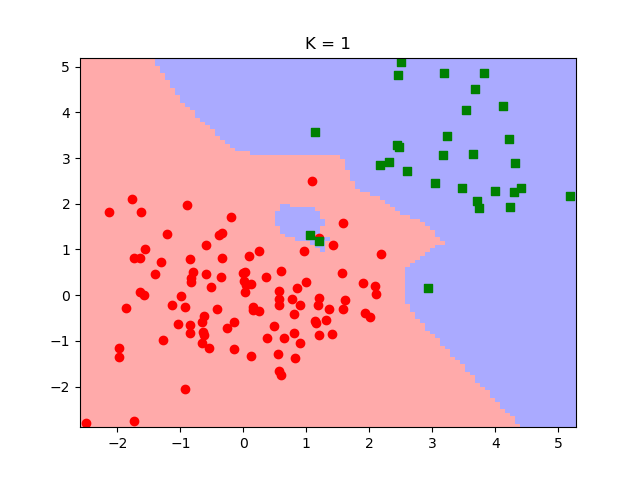
\includegraphics[width=\linewidth]{code/knn_binary_data-k-1.png}
 \caption{KNN k=1 binary classification}
\label{label}
\end{figure}

\begin{figure}[H]
\centering
  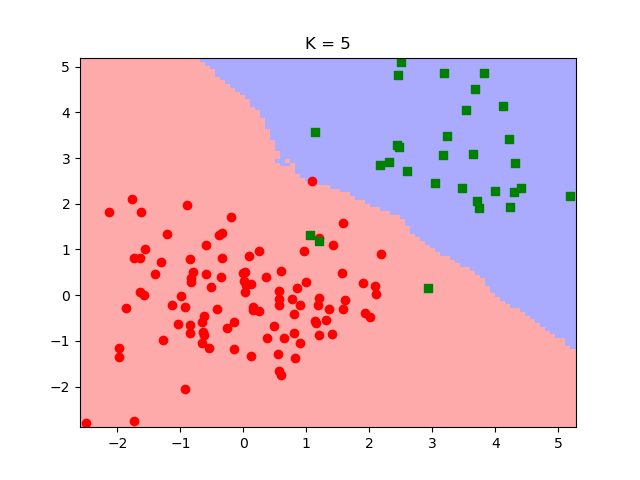
\includegraphics[width=\linewidth]{code/knn_binary_data-k-5.png}
 \caption{KNN k=5 binary classification}
\label{label}
\end{figure}

\begin{figure}[H]
\centering
  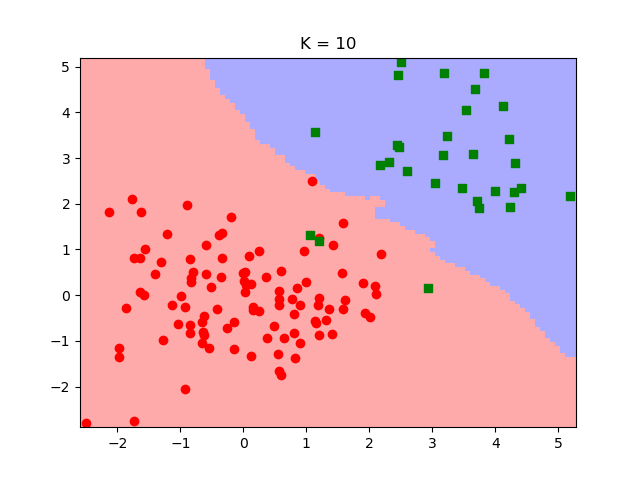
\includegraphics[width=\linewidth]{code/knn_binary_data-k-10.png}
 \caption{KNN k=10 binary classification}
\label{label}
\end{figure}

\begin{figure}[H]
\centering
  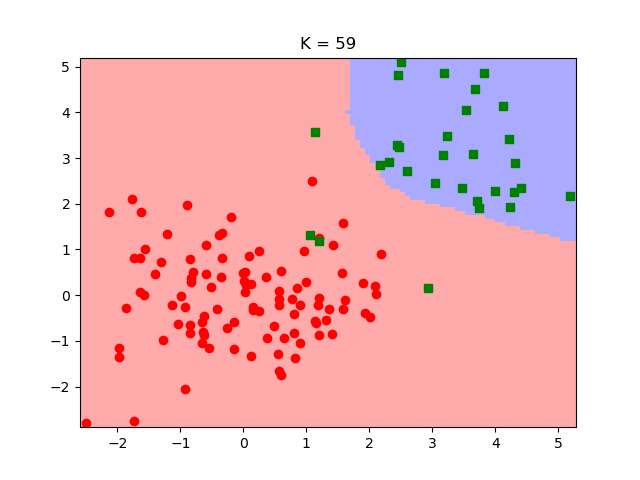
\includegraphics[width=\linewidth]{code/knn_binary_data-k-59.png}
 \caption{KNN k=59 binary classification}
\label{label}
\end{figure}

For the classification of three classes, k of 1 again is too liberal with creating boundaries for instance the one green square that is clearly in the red circle's area and also a red circle that ventures into the blue region. Again k of 5 and 10 create smoother boundaries that allow errant positions to wander where they ought not. K of 59 isn't actually terrible since there are roughly equal numbers of the three classes and so no one class gets marginalized too much, but it does a poorer job than 5 or 10.

\begin{figure}[H]
\centering
  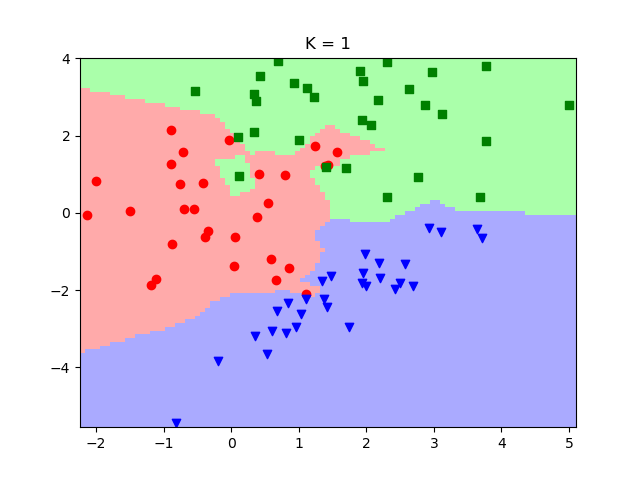
\includegraphics[width=\linewidth]{code/knn_three_class_data-k-1.png}
 \caption{KNN k=1 three class classification}
\label{label}
\end{figure}

\begin{figure}[H]
\centering
  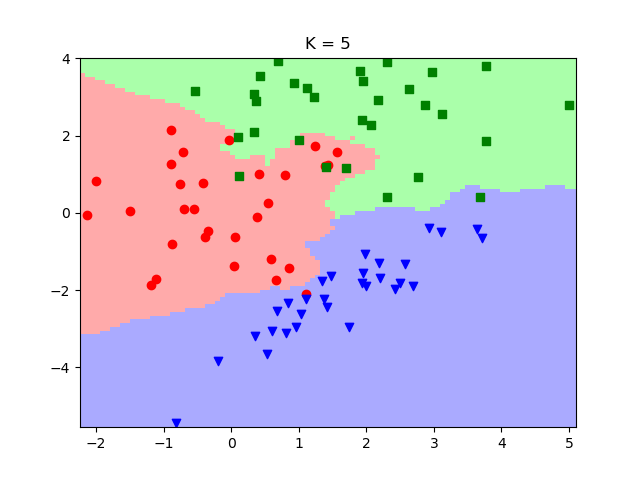
\includegraphics[width=\linewidth]{code/knn_three_class_data-k-5.png}
 \caption{KNN k=5 three class classification}
\label{label}
\end{figure}

\begin{figure}[H]
\centering
  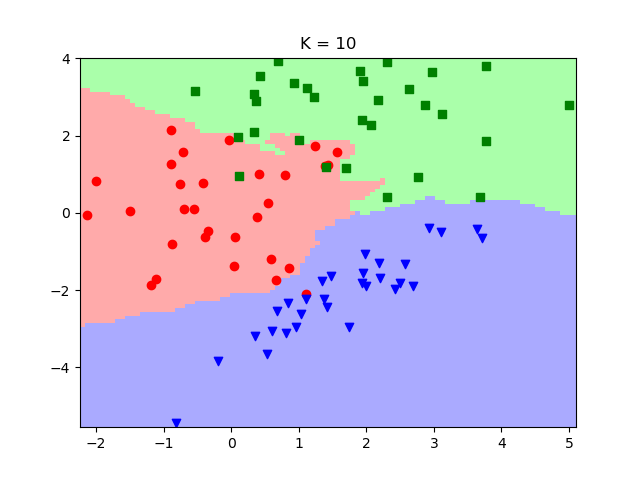
\includegraphics[width=\linewidth]{code/knn_three_class_data-k-10.png}
 \caption{KNN k=10 three class classification}
\label{label}
\end{figure}

\begin{figure}[H]
\centering
  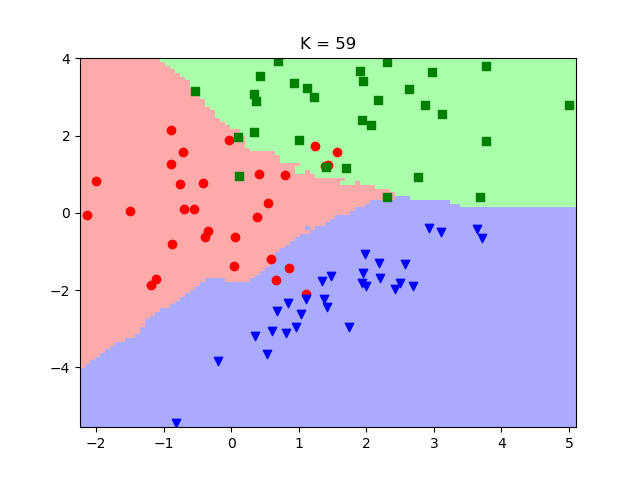
\includegraphics[width=\linewidth]{code/knn_three_class_data-k-59.png}
 \caption{KNN k=59 three class classification}
\label{label}
\end{figure}

\verbatiminput{./code/knn.py}

%%%     Problem 6
\item[6.]  [4 points]
Using your implementation of your KNN classifier in exercise 5, write a script to perform 10-fold cross-validation in a search for the best choice of $K$.  Remember to randomize your data at the start of the CV procedure, but use the same CV folds for each $K$.  Make your script search in the range of $1 \leq K \leq 30$.  Run your script on both data sources: {\tt knn\_binary\_data.csv} and {\tt knn\_three\_class\_data.csv}.  In your written solution, provide a plot of K (x-axis) to classification error (ratio of points misclassified to total; y-axis) for each data set, and report the \emph{best} k for each.  Submit your script as a python file named {\tt knn-cv}.

{\bf Solution.}

\begin{figure}[H]
\centering
  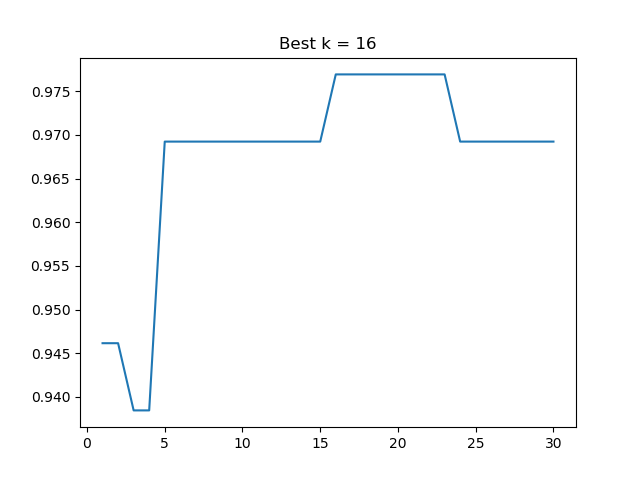
\includegraphics[width=\linewidth]{code/knn-cv-binary.png}
 \caption{10-fold cross validation of KNN on binary classification where 1 <= k <= 30}
\label{label}
\end{figure}

\begin{figure}[H]
\centering
  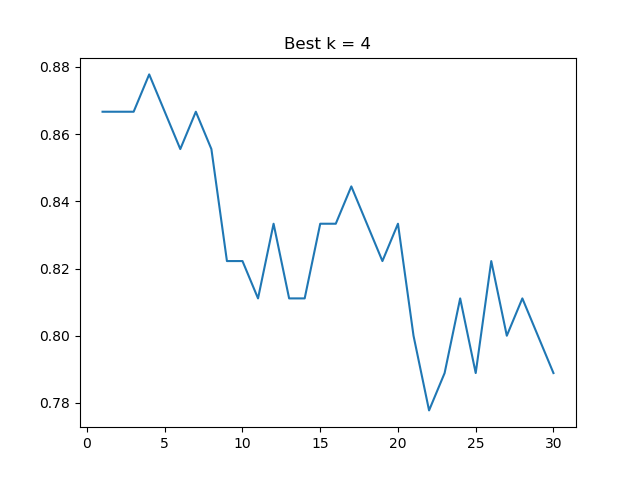
\includegraphics[width=\linewidth]{code/knn-cv-three.png}
 \caption{10-fold cross validation of KNN on three-class classification where 1 <= k <= 30}
\label{label}
\end{figure}

\verbatiminput{./code/knn-cv.py}

\end{itemize}

\end{document}
